\begin{center}
\Huge
	Inverse trigonometriske funktioner og arealformlen		
\end{center}

\section*{Inverse trigonometriske funktioner}
\stepcounter{section}

Vi husker os selv på, at for retvinklede trekanter $\triangle ABC$ som den på Figur \ref{fig:retvinklet}
har vi følgende sætning.
\begin{setn}
	Der gælder for retvinklede trekanter, at
	\begin{align*}
		\cos(v) &= \frac{\textnormal{hos}}{\textnormal{hyp}}, \\
		\sin(v) &= \frac{\textnormal{mod}}{\textnormal{hyp}}, \\
		\tan(v) &= \frac{\textnormal{mod}}{\textnormal{hos}}.
	\end{align*}
\end{setn}

\begin{figure}[H]
	\centering
	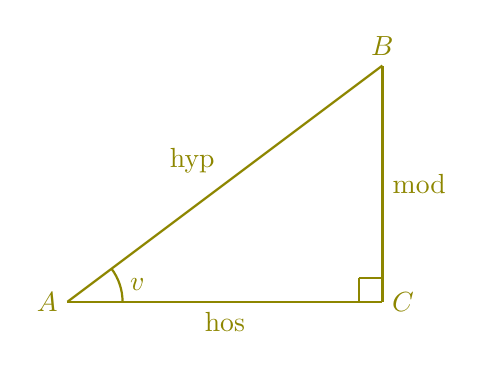
\begin{tikzpicture}
		\draw[color = olive, thick] (0,0) -- (4,0) node[midway, anchor = north] {hos};
		\draw[color = olive, thick] (0,0) -- (4,3) node[midway, anchor = south east] {hyp};
		\draw[color = olive, thick] (4,0) -- (4,3) node[midway, anchor = west] {mod};
		\draw[color = olive, thick] (0.7,0) arc (0:36.87:0.7) node[midway, anchor = west] {$v$};
		\draw[color = olive, thick] (3.7,0) to (3.7,0.3);
		\draw[color = olive, thick] (3.7,0.3) to (4,0.3);
		\node[color = olive, anchor = east] at (0,0) {$A$};
		\node[color = olive, anchor = west] at (4,0) {$C$};
		\node[color = olive, anchor = south] at (4,3) {$B$};
	\end{tikzpicture}
	\caption{Retvinklet trekant.}
	\label{fig:retvinklet}
\end{figure}

Kender vi vinklen $v$ samt én af siderne, så er det ligefrem at finde den sidste side. Så isoleres den ukendte side blot i udtrykket og vinklen indsættes i den passende trigonometriske funktion og enten aflæses i en tabel eller udregnes med et CAS-værktøj. Kender vi derimod ikke vinklen, så skal vi bruge den inverse funktion til den trigonometriske funktion. Disse skrives som sædvanligt $\cos^{-1}$, $\sin^{-1}$ og  $\tan^{-1}$.

Der er dog et vist problem. Vi husker på, at funktioner kun har inverse funktioner, hvis de er injektive. Betragter vi Figur \ref{fig:cossin}, så er hverken $\cos$ eller $\sin$ injektive. Derfor defineres de inverse funktioner på et begrænset interval, navnligt gælder der for definitionsmængderne, at 
\begin{align*}
	&\textnormal{Dm($\cos^{-1}$)} = [-1,1],\\
	&\textnormal{Dm($\sin^{-1}$)} = [-1,1].
\end{align*}
Dette giver os værdimængderne
\begin{align*}
	&\textnormal{Vm}(\cos^{-1}) = [0,180],\\
	&\textnormal{Vm}(\sin^{-1}) = [-90,90].
\end{align*}

\begin{figure}[H]
	\centering
	\begin{minipage}{0.45\textwidth}
	\centering
	\resizebox{0.99\textwidth}{!}
	{
	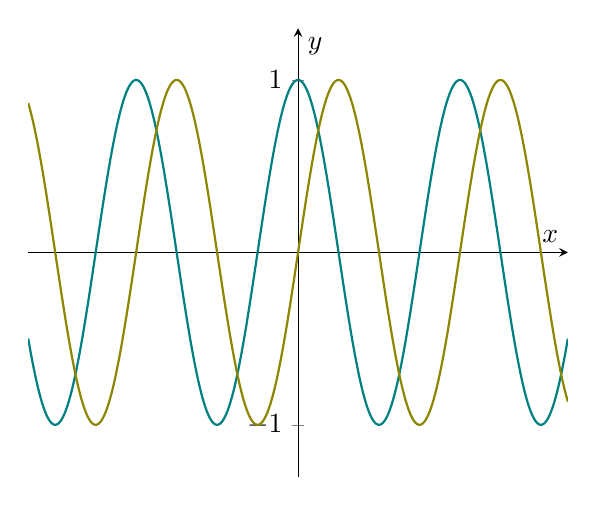
\begin{tikzpicture}
	\begin{axis}[
		axis lines = center, xmin = -600, xmax = 600, 
		ymin = -1.3, ymax = 1.3,
		xlabel = $x$, ylabel = $y$,
		xtick = {0}, ytick = {-1,1},
	]
		\addplot[color = teal, thick, domain = -600: 600, samples = 500] {cos(x)};
		\addplot[color = olive, thick, domain = -600: 600, samples = 500] {sin(x)};
	\end{axis}
	\end{tikzpicture}
	}
	\caption{Grafer for \textcolor{teal}{$\cos$} og \textcolor{olive}{$\sin$}.}
	\label{fig:cossin}
	\end{minipage}%
	\hfill
	\begin{minipage}{0.45\textwidth}
	\centering
	\resizebox{0.99\textwidth}{!}
	{
	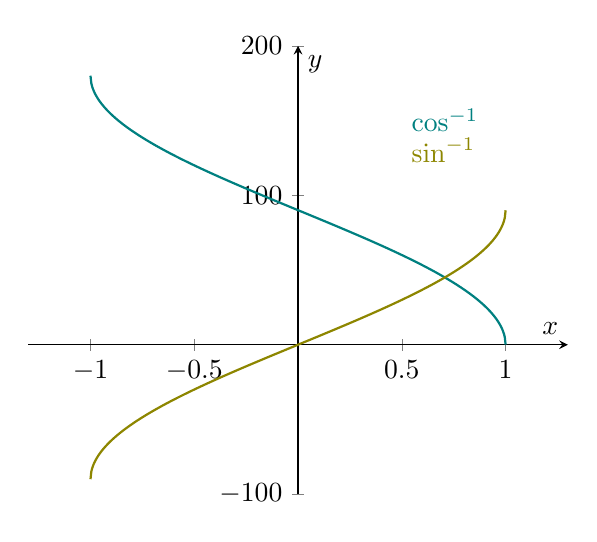
\begin{tikzpicture}
	\begin{axis}[
		axis lines = center, xmin = -1.3, xmax = 1.3, 
		ymin = -100, ymax = 200,
		xlabel = $x$, ylabel = $y$,
	]
		\addplot[color = teal, thick, domain = -1:1, samples = 500] {acos(x)};
		\addplot[color = olive, thick, domain = -1:1, samples = 500] {asin(x)};
		\node[color = teal, anchor = west] at (axis cs: 0.5,150) {$\cos^{-1}$};
		\node[color = olive, anchor = west] at (axis cs: 0.5,130) {$\sin^{-1}$};
	\end{axis}
	\end{tikzpicture}
	}
	\caption{Grafer for \textcolor{teal}{$\cos^{-1}$} og \textcolor{olive}{$\sin^{-1}$}.}
	\label{fig:invers}
	\end{minipage}%
	\hfill
\end{figure}

Vi betragter et eksempel.
\begin{exa}
	En $\triangle ABC$ trekant er givet ved følgende. 
	\begin{center}
	\begin{tikzpicture}
		\draw[color = olive, thick] (0,0) -- (6,0) node[midway, anchor = north] {$6$};
		\draw[color = olive, thick] (0,0) -- (6,4) node[midway, anchor = south east] {$c$};
		\draw[color = olive, thick] (6,0) -- (6,4) node[midway, anchor = west] {$4$};
		\draw[color = olive, thick] (0.7,0) arc (0:33.69:0.7) node[midway, anchor = west] {$v$};
		\draw[color = olive, thick] (6,0) rectangle (6-0.3,0.3);
		\node[color = olive, anchor = east] at (0,0) {$A$};
		\node[color = olive, anchor = west] at (6,0) {$C$};
		\node[color = olive, anchor = south] at (6,4) {$B$};
	\end{tikzpicture}
	\end{center}
	Vi kender den hosliggende og modstående katete. Skal vi finde vinklen $v$, skal vi derfor have fat i 
	$\tan^{-1}$. Vi får altså
	\begin{align*}
		\tan(v) = \frac{4}{6} \ &\Leftrightarrow \ v = \tan^{-1}\left(\frac{4}{6}\right).
	\end{align*}
	Dette udregnes med et CAS-værktøj og vi får
	\begin{align*}
		\tan^{-1}\left( \frac{4}{6} \right) = 33.69.
	\end{align*}
\end{exa}
Når vi skal bruge $\cos^{-1}$, $\sin^{-1}$ og $\tan^{-1}$ i Maple, så skal vi bruge et alternativt navn for funktionerne, navnligt $\arccos$, $\arcsin$ og $\arctan$, der udtales arcus cosinus, arcus sinus og arcus tangens. Mere præcist skriver vi i Maple:
\begin{align*}
	&\texttt{with(Gym):} \\
	&\texttt{arcTan(4/6.)}
\end{align*}
Dette vil så gives os resultatet $v = 33.69$. 

\section*{Arealformlen}
\stepcounter{section}

Det er også muligt at bestemme arealet for en trekant, hvis man kender to sider og den mellemliggende vinkel i stedet for højden på trekanten. Denne formel kaldes til tider for \textit{appelsin-formlen}, da formlen lyder lidt som en halv appelsin. Vi betragter trekanten på Figur \ref{fig:vilkårlig}.
\begin{figure}[H]
	\centering
	\begin{tikzpicture}
		\draw[color = olive, thick] (0,0) -- (5,0) node[midway, anchor = north] {$b$};
		\draw[color = olive, thick] (0,0) -- (4,3) node[midway, anchor = south east] {$c$};
		\draw[color = olive, thick] (5,0) -- (4,3) node[midway, anchor = west] {$a$};
		\node[color = olive, anchor = east] at (0,0) {$A$};
		\node[color = olive, anchor = west] at (5,0) {$C$};
		\node[color = olive, anchor = south] at (4,3) {$B$};
	\end{tikzpicture}
	\caption{Vilkårlig trekant $\triangle ABC$}
	\label{fig:vilkårlig}
\end{figure}
For trekanter som denne gælder der følgende sætning
\begin{setn}[Appelsin-formlen]
	For vilkårlige trekanter $\triangle ABC$ som den på Figur \ref{fig:vilkårlig} gælder der,
	 at arealet $M$ af trekanten er givet ved
	 \begin{align*}
	 	M = \frac{1}{2}ab \sin(\angle C).
	 \end{align*}
\end{setn}

\begin{exa}
En trekant $\triangle ABC$ er givet ved følgende
\begin{center}
	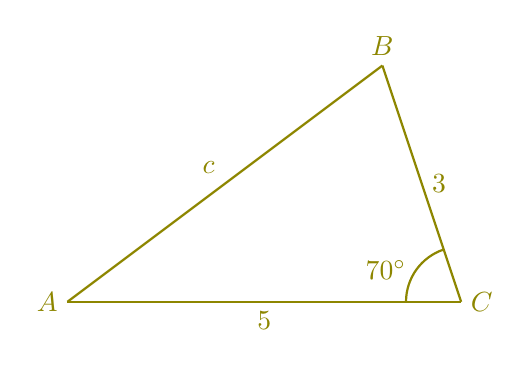
\begin{tikzpicture}
		\draw[color = olive, thick] (0,0) -- (5,0) node[midway, anchor = north] {$5$};
		\draw[color = olive, thick] (0,0) -- (4,3) node[midway, anchor = south east] {$c$};
		\draw[color = olive, thick] (5,0) -- (4,3) node[midway, anchor = west] {$3$};
		\draw[color = olive, thick] (4.3,0) arc (180:180-71.57:0.7) node[midway, anchor = east] {$70^{\circ}$};
		\node[color = olive, anchor = east] at (0,0) {$A$};
		\node[color = olive, anchor = west] at (5,0) {$C$};
		\node[color = olive, anchor = south] at (4,3) {$B$};
	\end{tikzpicture}
\end{center}
For at bestemme arealet, sætter vi ind i formlen. Vi får derfor
\begin{align*}
	M = \frac{1}{2}\cdot 3 \cdot 5 \cdot \sin(70) = 7.05
\end{align*}
og arealet af trekanten er derfor $M = 7.05$.
\end{exa}
\newpage
\begin{table}[H]
	\centering
	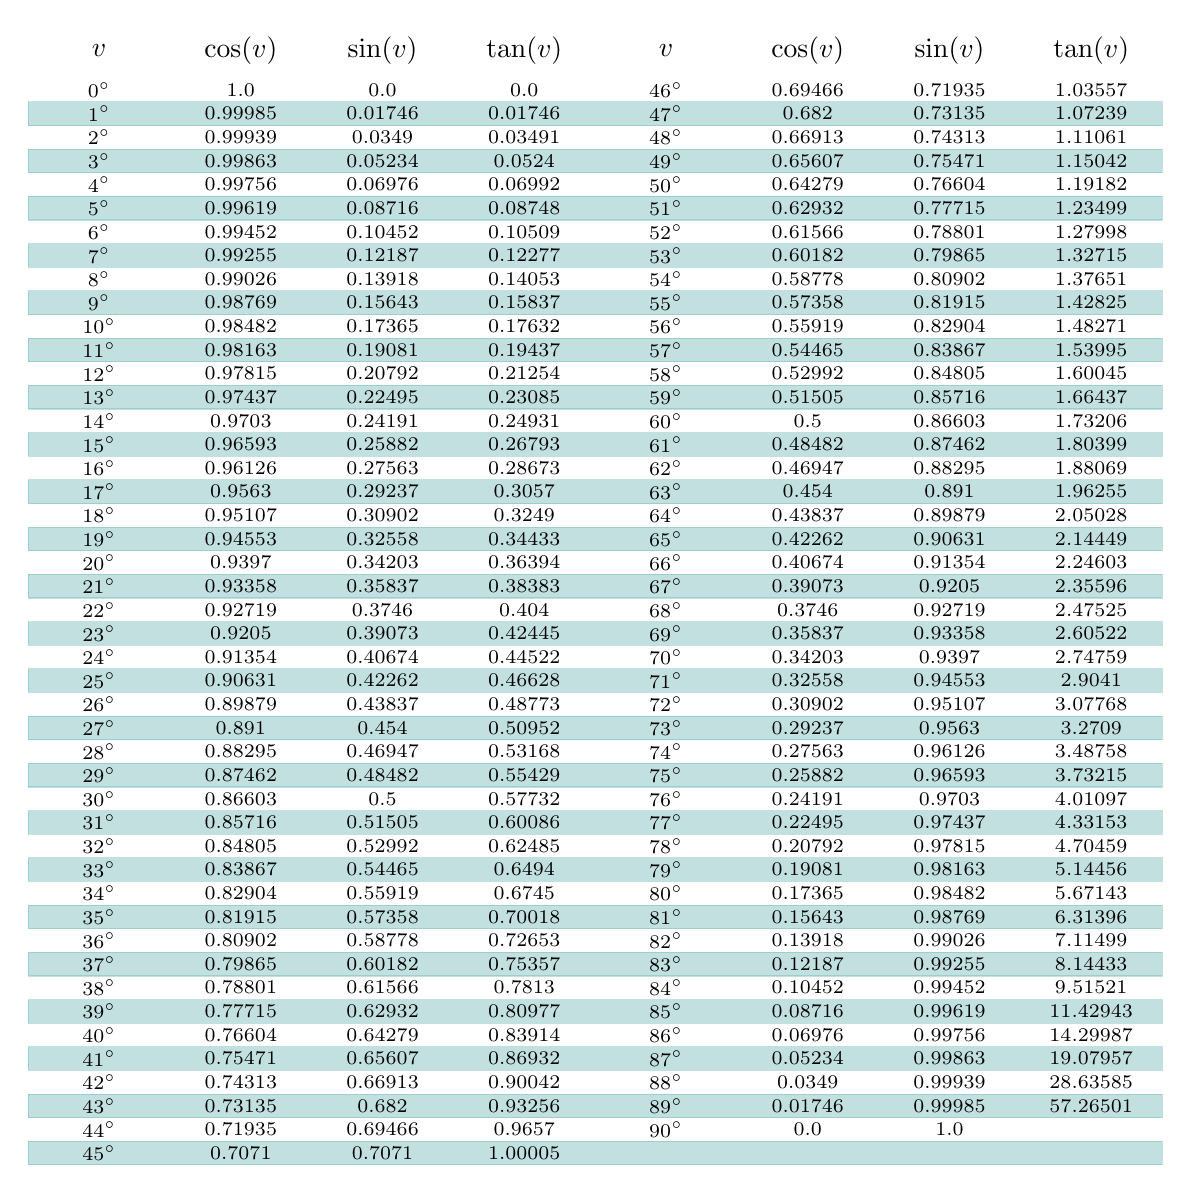
\begin{tikzpicture}
	\node at (0,0) {$v$};
	\node at (2*0.9,0) {$\cos(v)$};
	\node at (4*0.9,0) {$\sin(v)$};
	\node at (6*0.9,0) {$\tan(v)$};
	\node at (8*0.9,0) {$v$};
	\node at (10*0.9,0) {$\cos(v)$};
	\node at (12*0.9,0) {$\sin(v)$};
	\node at (14*0.9,0) {$\tan(v)$};
	\scriptsize
	%Colors
	\foreach \i in {0,...,22}{
		\filldraw[color = teal!60, opacity = 0.4] (-0.9,-0.5-0.3+0.15-\i*0.3*2) rectangle
		 (14*0.9 + 0.9,-0.5-0.3-0.15-\i*0.3*2);
	}
	\foreach \i in {0,...,45}{
		%Macros for evaluating
		\pgfmathsetmacro{\cval}{cos(\i)}
		\pgfmathsetmacro{\sval}{sin(\i)}
		\pgfmathsetmacro{\tval}{tan(\i)}
		%First columns of values
		\node at (0,-0.5-\i*0.3) {$\i^{\circ}$};
		\node at (2*0.9,-0.5-\i*0.3) { \cval };
		\node at (4*0.9,-0.5-\i*0.3) { \sval };
		\node at (6*0.9,-0.5-\i*0.3) { \tval };
	}
	\foreach \i in {46,...,89}{
		%Macros
		\pgfmathsetmacro{\cval}{cos(\i)}
		\pgfmathsetmacro{\sval}{sin(\i)}
		\pgfmathsetmacro{\tval}{tan(\i)}
		%Second column
		\node at (8*0.9,-0.5-\i*0.3 + 46*0.3) {$\i^{\circ}$};
		\node at (10*0.9,-0.5-\i*0.3 + 46*0.3) { \cval };
		\node at (12*0.9,-0.5-\i*0.3 + 46*0.3) { \sval };
		\node at (14*0.9,-0.5-\i*0.3 + 46*0.3) { \tval };
	}
		\pgfmathsetmacro{\cval}{cos(90)}
		\pgfmathsetmacro{\sval}{sin(90)}
		\node at (8*0.9,-0.5-90*0.3 + 46*0.3) {$90^{\circ}$};
		\node at (10*0.9,-0.5-90*0.3 + 46*0.3) { \cval };
		\node at (12*0.9,-0.5-90*0.3 + 46*0.3) { \sval };
	\end{tikzpicture}
	\caption{Tabel over udvalgte værdier for $\cos$, $\sin$ og $\tan$.}
	\label{tab:cossintan}
\end{table}

\newpage
\begin{figure}[H]
	\centering
	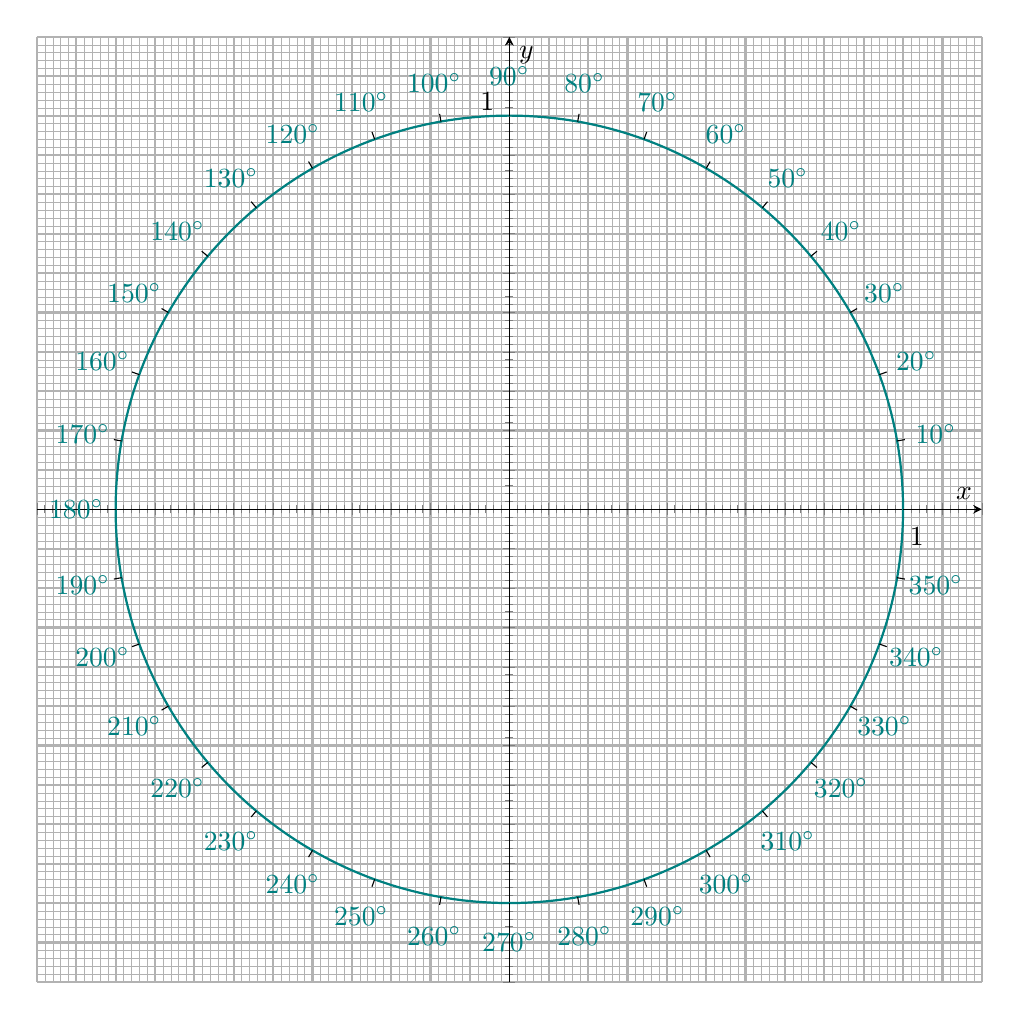
\begin{tikzpicture}
		\begin{axis}[
			axis lines = center, 
			xmin = -1.2, xmax = 1.2, 
			ymin = -1.2, ymax = 1.2, 
			x = 5cm, y = 5cm,
			major grid style={line width=0.8pt, draw=gray!60},
			minor grid style={line width=0.1pt, draw=gray!60},
			ytick distance = 0.1,
			xtick distance = 0.1,
			minor tick num = 4,
			grid = both,
			xticklabels = {},
			yticklabels = {},
			xlabel = $x$, ylabel = $y$
		]
			%Shifted tick labels since unit circle would otherwise be in the way:
			\node[xshift = 5pt, yshift = -10pt] at (axis cs:1,0) {1};
			\node[xshift = -8pt, yshift = 5pt] at (axis cs:0,1) {1};
			\draw[color = teal, thick] (axis cs:0,0) circle (5cm);
			%Ticks on circle 
			\pgfplotsinvokeforeach{0,1,...,35}
			{
				\draw (axis cs: {cos(#1*10)},{sin(#1*10)})-- (axis cs: {1.02*cos(#1*10)},{1.02*sin(#1*10)});
			}
			\pgfplotsinvokeforeach{10,20,...,350}
			{
				\node[color = teal] at (axis cs: {1.10*cos(#1)},{1.10*sin(#1)}) {$#1^\circ$};
			}
		\end{axis}
	\end{tikzpicture}
	\caption{Enhedscirkel til aflæsning af $\cos$ og $\sin$.}
	\label{fig:enhed}
\end{figure}

\newpage

\subsection*{Opgave 1}

Brug Figur \ref{fig:enhed} til at bestemme følgende
\begin{align*}
	&1) \ \cos(45)    &     &2) \ \sin(170) \\
	&3) \ \sin^{-1}(0.7) &  &4) \ \cos^{-1}(0.32) \\
	&5) \ \cos^{-1}(-1)  &  &6) \ \sin^{-1}(0.32) \\
	&7) \ \sin(250)      &  &8) \ \cos(300) \\
	&9) \ \cos^{-1}(-0.2)&  &10) \ \sin^{-1}(-0.6) \\
\end{align*}

\subsection*{Opgave 2}

Brug tabel \ref{tab:cossintan} til at bestemme vinklen i følgende trekanter. Tjek desuden dit resultat i Maple. 

\begin{center}
	\begin{minipage}{0.45\textwidth}
		\centering
		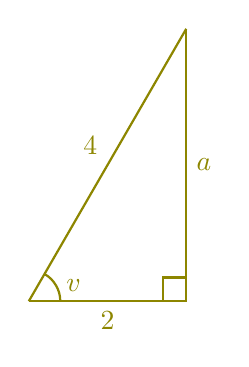
\begin{tikzpicture}
		\draw[color = olive, thick] (0,0) -- (2,0) node[midway, anchor = north] {$2$};
		\draw[color = olive, thick] (0,0) -- (2,3.46) node[midway, anchor = south east] {$4$};
		\draw[color = olive, thick] (2,0) -- (2,3.46) node[midway, anchor = west] {$a$};
		\draw[color = olive, thick] (0.4,0) arc (0:60:0.4) node[midway, anchor = west] {$v$};
		\draw[color = olive, thick] (2,0) rectangle (2-0.3,0.3);
		\end{tikzpicture}
	\end{minipage}
	\begin{minipage}{0.45\textwidth}
		\centering
		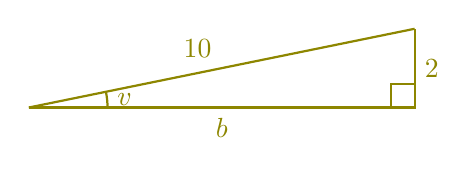
\begin{tikzpicture}
		\draw[color = olive, thick] (0,0) -- (4.9,0) node[midway, anchor = north] {$b$};
		\draw[color = olive, thick] (0,0) -- (4.9,1) node[midway, anchor = south east] {$10$};
		\draw[color = olive, thick] (4.9,0) -- (4.9,1) node[midway, anchor = west] {$2$};
		\draw[color = olive, thick] (1,0) arc (0:11.52:1) node[midway, anchor = west] {$v$};
		\draw[color = olive, thick] (4.9,0) rectangle (4.9-0.3,0.3);
		\end{tikzpicture}
	\end{minipage}
	\begin{minipage}{0.45\textwidth}
		\centering
		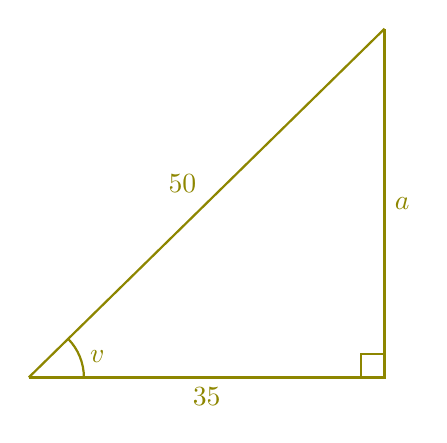
\begin{tikzpicture}
		\draw[color = olive, thick] (0,0) -- (7.53*0.6,0) node[midway, anchor = north] {$35$};
		\draw[color = olive, thick] (0,0) -- (7.53*0.6,7.38*0.6) node[midway, anchor = south east] {$50$};
		\draw[color = olive, thick] (7.53*0.6,0) -- (7.53*0.6,7.38*0.6) node[midway, anchor = west] {$a$};
		\draw[color = olive, thick] (0.7,0) arc (0:44.43:0.7) node[midway, anchor = west] {$v$};
		\draw[color = olive, thick] (7.53*0.6,0) rectangle (7.53*0.6-0.3,0.3);
		\end{tikzpicture}
	\end{minipage}
	\begin{minipage}{0.45\textwidth}
		\centering
		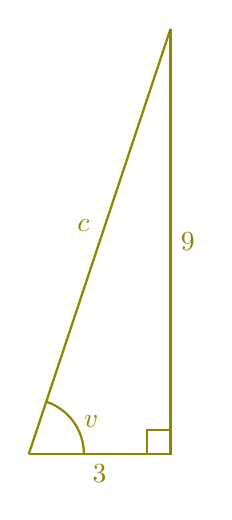
\begin{tikzpicture}
		\pgfmathsetmacro{\hos}{3*0.6}
		\pgfmathsetmacro{\mod}{9*0.6}
		\pgfmathsetmacro{\vinkel}{atan(\mod / \hos)}
		
		\draw[color = olive, thick] (0,0) -- (\hos,0) node[midway, anchor = north] {$3$};
		\draw[color = olive, thick] (0,0) -- (\hos,\mod) node[midway, anchor = south east] {$c$};
		\draw[color = olive, thick] (\hos,0) -- (\hos,\mod) node[midway, anchor = west] {$9$};
		\draw[color = olive, thick] (0.7,0) arc (0:\vinkel:0.7) node[midway, anchor = west] {$v$};
		\draw[color = olive, thick] (\hos,0) rectangle (\hos-0.3,0.3);
		\end{tikzpicture}
	\end{minipage}
\end{center}

\subsection*{Opgave 3}

Vi skal overbevise os selv om, at vinklerne $1^\circ, 2^\circ, \hdots, 90^\circ$ er nok i Tabel \ref{tab:cossintan}. Dette gøres i disse delopgaver. Bestem derfor følgende ved at bruge Tabel \ref{tab:cossintan}.

\begin{align*}
	&1) \ \cos(95)   &  &2) \sin(102) \\
	&3) \ \cos(-10)  &  &4) \sin(242) \\
	&5) \ \cos(295)  &  &6) \sin(-116) \\
	&7) \ \cos(-351)  &  &8) \sin(517) \\
	&9) \ \cos(166)  &  &10) \sin(-50) \\	
\end{align*}

Vi kan generalisere dette. For to forskellige vinkler $u$ og $v$, hvad skal der så gælde for disse vinkler for, at følgende gælder. Brug evt. enhedscirklen til at hjælpe dig. 
\begin{enumerate}[label=\roman*)]
	\item $\cos(u) = \cos(v)$.
	\item $\sin(u) = \sin(v)$.
	\item $\cos(u) = -\cos(v)$.
	\item $\sin(u) = -\sin(v)$.
\end{enumerate}

\subsection*{Opgave 4 (med hjælpemidler)}

For en retvinklet trekant $\triangle ABC$ med $\angle C = 90^\circ$ gælder der, at $a = 6$ og $c = 15$.
\begin{enumerate}[label=\roman*)	]
	\item Tegn en skitse af $\triangle ABC$. 
	\item Bestem $\angle A$ uden at bruge \textit{solve}.
\end{enumerate}

\subsection*{Opgave 5 (med hjælpemidler)}

For en retvinklet trekant $\triangle ABC$ med $\angle C = 90^\circ$ gælder der, at $b = 6$ og $\angle B = 70^\circ$.
\begin{enumerate}[label=\roman*)	]
	\item Tegn en skitse af $\triangle ABC$. 
	\item Bestem længden af de resterende sider uden at bruge \textit{solve}.
\end{enumerate}

\subsection*{Opgave 6 (med hjælpemidler)}

For en retvinklet trekant $\triangle ABC$ med $\angle C = 90^\circ$ gælder der, at $b = 6$ og arealet af trekanten er 40.
\begin{enumerate}[label=\roman*)	]
	\item Tegn en skitse af $\triangle ABC$. 
	\item Bestem $\angle A$ uden at bruge \textit{solve}.
	\item Bestem længden af de resterende sider. 
\end{enumerate}

\subsection*{Opgave 7}

Bestem arealet af trekant $\triangle ABC$ ved at bruge Tabel \ref{tab:cossintan}.

\begin{center}
	\begin{tikzpicture}
		\draw[color = olive, thick] (-7,0) -- (0,0) node[midway, anchor = south] {$5$};
		\draw[color = olive, thick] (-5.2,-3) -- (0,0) node[midway, anchor = north west] {$6$};
		\draw[color = olive, thick] (-7,0) -- (-5.2,-3) node[midway, anchor = east] {$c$};
		\draw[color = olive, thick] (-0.7,0) arc (180:210:0.7) node[midway, anchor = east] {$30^{\circ}$};
		\node[color = olive, anchor = east] at (-7,0) {$A$};
		\node[color = olive, anchor = west] at (0,0) {$C$};
		\node[color = olive, anchor = north] at (-5.2,-3) {$B$};
	\end{tikzpicture}
\end{center}

\subsection*{Opgave 8 (med hjælpemidler)}

En trekant $\triangle ABC$ har $\angle C = 50$, $a = 10$ og $b = 7$
\begin{enumerate}[label=\roman*)]
	\item Bestem arealet af $\triangle ABC$
\end{enumerate}

\subsection*{Opgave 9 (med hjælpemidler)}
En trekant $\triangle ABC$ har $\angle A = 120$, $b = 5$ og et areal på 19.
\begin{enumerate}[label=\roman*)]
	\item Tegn en skitse af $\triangle ABC$.
	\item Bestem sidelængden $c$. 
\end{enumerate}

\subsection*{Opgave 10}

Vi skal i denne opgave bevise idiotformlen $\cos(v)^2 + \sin(v)^2 = 1$.

\begin{enumerate}[label=\roman*)]
	\item Tegn en retvinklet trekant, hvor hypotenusen er linjestykket fra centrum af enhedscirklen til 
	punktet $P_v$ på kanten af enhedscirklen. 
	\item Hvad er længden af hypotenusen og de to kateter i denne trekant?
	\item Anvend Pythagoras' læresætning på denne trekant.
\end{enumerate}

\subsection*{Opgave 11}

Brug idiotformlen til at bestemme $\cos(45)$ eksakt.

